\hypertarget{ux57faux4e8eux4ef7ux503cux7684ux5f3aux5316ux5b66ux4e60}{%
\chapter{基于价值的强化学习}\label{ux57faux4e8eux4ef7ux503cux7684ux5f3aux5316ux5b66ux4e60}}

\hypertarget{ux8499ux7279ux5361ux6d1bux65b9ux6cd5}{%
\section{蒙特卡洛方法}\label{ux8499ux7279ux5361ux6d1bux65b9ux6cd5}}

基于价值的强化学习，即学习一个价值函数，根据价值函数选择策略。其关键在于如何求解价值函数。

蒙特卡洛方法（Monte-Carlo methods）也被称为统计模拟方法，是一种基于概率统计的数值计算方法。运用蒙特卡洛方法时，我们通常使用重复随机抽样，然后运用概率统计方法来从抽样结果中归纳出我们想求的目标的数值估计。一个简单的例子是用蒙特卡洛方法来计算圆的面积。例如，在正方形内部随机产生若干个点，细数落在圆中点的个数，圆的面积与正方形面积之比就等于圆中点的个数与正方形中点的个数之比。如果我们随机产生的点的个数越多，计算得到圆的面积就越接近于真实的圆的面积。用蒙特卡洛方法可以估计一个策略在一个马尔可夫决策过程中的状态价值函数。一个状态的价值是它的期望回报，那么一个很直观的想法就是用策略在 MDP 上采样很多条序列，计算从这个状态出发的回报再求其期望就可以了，公式如下：

\[
V^\pi(s)=\mathbb{E}_\pi[G_t|S_t=s]\approx \frac{1}{N}\sum_{i=1}^{N}G_t^{(i)}
\]

在一条序列中，可能没有出现过这个状态，可能只出现过一次这个状态，也可能出现过很多次这个状态。蒙特卡洛价值估计方法会在该状态每一次出现时计算它的回报。还有一种选择是一条序列只计算一次回报，也就是这条序列第一次出现该状态时计算后面的累积奖励，而后面再次出现该状态时，该状态就被忽略了。假设我们现在用策略 \(\pi\) 从状态 \(s\) 开始采样序列，据此来计算状态价值。我们为每一个状态维护一个计数器和总回报，计算状态价值的具体过程如下所示。

（1）使用策略 \(\pi\) 采样若干条序列：

\[
s_0^{(i)} \xrightarrow{a_0^{(i)}} r_0^{(i)},s_1^{(i)} \xrightarrow{a_1^{(i)}} r_1^{(i)},s_2^{(i)} \xrightarrow{a_2^{(i)}} \cdots \xrightarrow{a_{T-1}^{(i)}} r_{T-1}^{(i)},s_T^{(i)}
\]

（2）对每一条序列中的每一时间步的状态 \(s\) 进行以下操作：

\begin{itemize}
\tightlist
\item
  更新状态 \(s\) 的计数器 \(N(s)\leftarrow N(s)+1\)；
\item
  更新状态 \(s\) 的总回报 \(M(s)\leftarrow M(s)+G_t\)；
\end{itemize}

（3）每一个状态的价值被估计为回报的平均值 \(V(s)=M(s)/N(s)\)。

根据大数定律，当 \(N(s)\to\infty\)，有 \(V(s)\to V^\pi(s)\)。计算回报的期望时，除了可以把所有的回报加起来除以次数，还有一种增量更新的方法。对于每个状态 \(s\) 和对应回报 \(G\)，进行如下计算：

\begin{itemize}
\tightlist
\item
  \(N(s)\leftarrow N(s)+1\)
\item
  \(V(s)\leftarrow V(s)+\frac{1}{N(s)}(G-V(s))\)
\end{itemize}

\hypertarget{ux53c2ux8003ux6587ux732e-44}{%
\subsection{参考文献}\label{ux53c2ux8003ux6587ux732e-44}}

\begin{itemize}
\tightlist
\item
  \href{https://hrl.boyuai.com/}{《动手学强化学习》}.
\end{itemize}

\clearpage

\hypertarget{ux52a8ux6001ux89c4ux5212ux7b97ux6cd5}{%
\section{动态规划算法}\label{ux52a8ux6001ux89c4ux5212ux7b97ux6cd5}}

动态规划（dynamic programming）是程序设计算法中非常重要的内容，能够高效解决一些经典问题，例如背包问题和最短路径规划。动态规划的基本思想是将待求解问题分解成若干个子问题，先求解子问题，然后从这些子问题的解得到目标问题的解。动态规划会保存已解决的子问题的答案，在求解目标问题的过程中，需要这些子问题答案时就可以直接利用，避免重复计算。本章介绍如何用动态规划的思想来求解在马尔可夫决策过程中的最优策略。

基于动态规划的强化学习算法可以在已知环境状态转移和奖励对的情况下求解策略，主要有两种：一是策略迭代（policy iteration），二是价值迭代（value iteration）。其中，策略迭代由两部分组成：策略评估（policy evaluation）和策略提升（policy improvement）。具体来说，策略迭代中的策略评估使用贝尔曼期望方程来得到一个策略的状态价值函数，这是一个动态规划的过程；而价值迭代直接使用贝尔曼最优方程来进行动态规划，得到最终的最优状态价值。

不同于前面介绍的蒙特卡洛方法和后面介绍的时序差分算法，基于动态规划的这两种强化学习算法要求事先知道环境的状态转移函数和奖励函数，也就是需要知道整个马尔可夫决策过程。在这样一个白盒环境中，不需要通过智能体和环境的大量交互来学习，可以直接用动态规划求解状态价值函数。但是，现实中的白盒环境很少，这也是动态规划算法的局限之处，我们无法将其运用到很多实际场景中。另外，策略迭代和价值迭代通常只适用于有限马尔可夫决策过程，即状态空间和动作空间是离散且有限的。

\hypertarget{ux7b56ux7565ux8fedux4ee3sarsa-ux7684ux57faux7840}{%
\subsubsection{1. 策略迭代（Sarsa 的基础）}\label{ux7b56ux7565ux8fedux4ee3sarsa-ux7684ux57faux7840}}

（1）策略评估

策略评估这一过程用来计算一个策略的状态价值函数。回顾一下之前学习的贝尔曼期望方程：

\[
V^{\pi}(s)=\sum_{a\in A}\pi(a|s)(r(s,a)+\gamma\sum_{s'\in S}p(s'|s,a)V^{\pi}(s'))
\]

其中，\(\pi(a|s)\) 是策略 \(\pi\) 在状态 \(s\) 下采取动作 \(a\) 的概率。可以看到，当知道奖励函数和状态转移函数时，我们可以根据下一个状态的价值来计算当前状态的价值。因此，根据动态规划的思想，可以把计算下一个可能状态的价值当成一个子问题，把计算当前状态的价值看作当前问题。在得知子问题的解后，就可以求解当前问题。更一般地，考虑所有的状态，就变成了用上一轮的状态价值函数来计算当前这一轮的状态价值函数，即

\[
V^{k+1}(s)=\sum_{a\in A}\pi(a|s)(r(s,a)+\gamma\sum_{s'\in S}P(s'|s,a)V^{k}(s'))
\]

我们可以选定任意初始值 \(V^{0}\)。根据贝尔曼期望方程，可以得知 \(V^{k}=V^{\pi}\) 是以上更新公式的一个不动点（fixed point）。事实上，可以证明当 \(k\to\infty\) 时，序列 \(\{V^{k}\}\) 会收敛到 \(V^{\pi}\)，所以可以据此来计算得到一个策略的状态价值函数。可以看到，由于需要不断做贝尔曼期望方程迭代，策略评估其实会耗费很大的计算代价。在实际的实现过程中，如果某一轮 \(\max_{s\in S}|V^{k+1}(s)-V^{k}(s)|\) 的值非常小，可以提前结束策略评估。这样做可以提升效率，并且得到的价值也非常接近真实的价值。

（2）策略提升

使用策略评估计算得到当前策略的状态价值函数之后，我们可以据此来改进该策略。假设此时对于策略 \(\pi\)，我们已经知道其价值 \(V^{\pi}\)，也就知道了在策略 \(\pi\) 下从每一个状态 \(s\) 出发最终得到的期望回报。我们要如何改变策略来获得在状态 \(s\) 下更高的期望回报呢？假设智能体在状态 \(s\) 下采取动作 \(a\)，之后的动作依旧遵循策略 \(\pi\)，此时得到的期望回报其实就是动作价值 \(Q^{\pi}(s,a)\)。如果我们有 \(Q^{\pi}(s,a)>V^{\pi}(s)\)，则说明在状态 \(s\) 下采取动作 \(a\) 会比原来的策略 \(\pi(a|s)\) 得到更高的期望回报。以上假设只是针对一个状态，现在假设存在一个确定性策略 \(\pi'\)，在任意一个状态 \(s\) 下，都满足

\[
Q^{\pi}(s,\pi'(s))\ge V^{\pi}(s)
\]

于是在任意状态 \(s\) 下，我们有

\[
V^{\pi'}(s)\ge V^{\pi}(s)
\]

这便是策略提升定理（policy improvement theorem）。于是我们可以直接贪心地在每一个状态选择动作价值最大的动作，也就是

\[
\pi'(s)=\arg\max_a Q^{\pi}(s,a)=\arg\max_a\bigl(r(s,a)+\gamma\sum_{s'}P(s'|s,a)V^{\pi}(s')\bigr)
\]

我们发现构造的贪心策略 \(\pi'\) 满足策略提升定理的条件，所以策略 \(\pi'\) 能够比策略 \(\pi\) 更好或者至少与其一样好。这个根据贪心法选取动作从而得到新的策略的过程称为策略提升。当策略提升之后得到的策略 \(\pi'\) 和之前的策略 \(\pi\) 一样时，说明策略迭代达到了收敛，此时 \(\pi\) 和 \(\pi'\) 就是最优策略。

策略提升定理的证明通过以下推导过程可以证明，使用上述提升公式得到的新策略 \(\pi'\) 在每个状态的价值不低于原策略 \(\pi\) 在该状态的价值。

\[
\begin{aligned}
V^{\pi}(s) &\le Q^{\pi}(s,\pi'(s))\\
&= \mathbb{E}_{\pi'}[R_t+\gamma V^{\pi}(S_{t+1})|S_t=s]\\
&\le \mathbb{E}_{\pi'}[R_t+\gamma Q^{\pi}(S_{t+1},\pi'(S_{t+1}))|S_t=s]\\
&= \mathbb{E}_{\pi'}[R_t+\gamma R_{t+1}+\gamma^{2}V^{\pi}(S_{t+2})|S_t=s]\\
&\le \mathbb{E}_{\pi'}[R_t+\gamma R_{t+1}+\gamma^{2}R_{t+2}+\gamma^{3}V^{\pi}(S_{t+3})|S_t=s]\\
&\vdots\\
&\le \mathbb{E}_{\pi'}[R_t+\gamma R_{t+1}+\gamma^{2}R_{t+2}+\gamma^{3}R_{t+3}+\cdots|S_t=s]\\
&= V^{\pi'}(s)
\end{aligned}
\]

可以看到，推导过程中的每一个时间步都用到局部动作价值优势 \(V^{\pi}(S_{t+1})\le Q^{\pi}(S_{t+1},\pi'(S_{t+1}))\)，累加到无穷步或者终止状态时，我们就得到了整个策略价值提升的不等式。

（3）策略迭代

总体来说，策略迭代算法的过程如下：对当前的策略进行策略评估，得到其状态价值函数，然后根据该状态价值函数进行策略提升以得到一个更好的新策略，接着继续评估新策略、提升策略，直到最后收敛到最优策略（收敛性证明参见 4.7 节）：

\[
\pi^{0} \xrightarrow{\mathcjk{策略评估}} V^{\pi^{0}} \xrightarrow{\mathcjk{策略提升}} \pi^{1} \xrightarrow{\mathcjk{策略评估}} V^{\pi^{1}} \xrightarrow{\mathcjk{策略提升}} \pi^{2} \xrightarrow{\mathcjk{策略评估}} \cdots \xrightarrow{\mathcjk{策略提升}} \pi^{*}
\]

结合策略评估和策略提升，我们得到以下策略迭代算法：

\begin{itemize}
\tightlist
\item
  随机初始化策略 \(\pi(s)\) 和价值函数 \(V(s)\)。
\item
  当 \(\Delta>\theta\) 时执行策略评估循环：

  \begin{itemize}
  \tightlist
  \item
    \(\Delta\leftarrow 0\)
  \item
    对于每一个状态 \(s\in S\)：

    \begin{itemize}
    \tightlist
    \item
      \(v\leftarrow V(s)\)
    \item
      \(V(s)\leftarrow r(s,\pi(s))+\gamma\sum_{s'}P(s'|s,\pi(s))V(s')\)
    \item
      \(\Delta\leftarrow \max(\Delta,|v-V(s)|)\)
    \end{itemize}
  \end{itemize}
\item
  结束策略评估循环后，令 \(\pi_{old}\leftarrow\pi\)。
\item
  对于每一个状态 \(s\in S\)：

  \begin{itemize}
  \tightlist
  \item
    \(\pi(s)\leftarrow \arg\max_a r(s,a)+\gamma\sum_{s'}P(s'|s,a)V(s')\)
  \end{itemize}
\item
  若 \(\pi_{old}=\pi\)，则停止算法并返回 \(V\) 和 \(\pi\)；否则转到策略评估循环。
\end{itemize}

和Sarsa的关系：

策略评估时，假设按当前策略，在 \(s\) 状态下采取动作 \(a\) 的价值为：

\[
Q^{\pi}(s,a)=\sum_{s'}P(s'|s,a)[R(s,a)+\gamma Q^{\pi}(s',\pi(s'))]
\]

注意：这里用的是 \(Q^{\pi}(s',\pi(s'))\) 或者 \(\sum_{a'}\pi(a'|s')Q(s',a')\)，而不是 \(\max_{a'}Q(s',a')\)。它老老实实计算当前策略的表现。

这里 \(\pi(s')\) 表示假设下一步仍然按同策略（更新前的策略）走时的 \(Q\)。

然后策略改进时再贪婪更新。

而在 Sarsa 中，我们不知道 \(P(s'|s,a)\) 的分布，因此无法求期望，只能用``采样+移动平均''：

Sarsa 是 State-Action-Reward-State-Action 的缩写。它的更新公式如下：

\[
Q(s,a)\leftarrow Q(s,a)+\alpha[\underbrace{R+\gamma Q(s',a')}_{\text{TD Target}}-Q(s,a)]
\]

\begin{itemize}
\tightlist
\item
  关系揭秘：

  \begin{itemize}
  \tightlist
  \item
    Sarsa 的目标 \(R+\gamma Q(s',a')\) 使用的是智能体实际采取的下一个动作 \(a'\)。
  \item
    这意味着 Sarsa 在估算的是当前策略 \(\pi\) 的价值 \(Q^{\pi}\)，而不是最优价值 \(Q^{*}\)。这对应了 PI 中的``策略评估''步骤。
  \item
    随着训练进行，我们通常会逐渐减小 \(\epsilon\)（让策略变得越来越贪婪）。这个过程让策略不断变好。这对应了 PI 中的``策略改进''步骤。
  \end{itemize}
\end{itemize}

\hypertarget{ux4ef7ux503cux8fedux4ee3q-learning-ux7684ux57faux7840}{%
\subsubsection{2. 价值迭代（Q-Learning 的基础）}\label{ux4ef7ux503cux8fedux4ee3q-learning-ux7684ux57faux7840}}

确切来说，价值迭代可以看成一种动态规划过程，它利用的是贝尔曼最优方程：

\[
V^{*}(s)=\max_{a\in A}\bigl(r(s,a)+\gamma\sum_{s'\in S}P(s'|s,a)V^{*}(s')\bigr)
\]

将其写成迭代更新的方式为

\[
V^{k+1}(s)=\max_{a\in A}\bigl(r(s,a)+\gamma\sum_{s'\in S}P(s'|s,a)V^{k}(s')\bigr)
\]

价值迭代便是按照以上更新方式进行的。等到 \(V^{k+1}\) 和 \(V^{k}\) 相同时，它就是贝尔曼最优方程的不动点，此时对应着最优状态价值函数 \(V^{*}\)。然后我们利用 \(\pi(s)=\arg\max_a(r(s,a)+\gamma\sum_{s'}p(s'|s,a)V^{k+1}(s'))\)，从中恢复出最优策略即可。

价值迭代算法流程如下：

\begin{itemize}
\tightlist
\item
  随机初始化 \(V(s)\)。
\item
  当 \(\Delta>\theta\) 时：

  \begin{itemize}
  \tightlist
  \item
    \(\Delta\leftarrow 0\)
  \item
    对于每一个状态 \(s\in S\)：

    \begin{itemize}
    \tightlist
    \item
      \(v\leftarrow V(s)\)
    \item
      \(V(s)\leftarrow \max_a r(s,a)+\gamma\sum_{s'}P(s'|s,a)V(s')\)
    \item
      \(\Delta\leftarrow \max(\Delta,|v-V(s)|)\)
    \end{itemize}
  \end{itemize}
\item
  结束循环后，返回一个确定性策略 \(\pi(s)=\arg\max_a(r(s,a)+\gamma\sum_{s'}P(s'|s,a)V(s'))\)。
\end{itemize}

和Q-Learning的关系：

在已知环境模型（转移概率 \(P\) 和奖励 \(R\)）的情况下，VI 通过迭代直接计算最优动作价值函数 \(Q^{*}(s,a)\)。更新公式（利用期望）为：

\[
Q_{k+1}(s,a)=\sum_{s'}P(s'|s,a)[R(s,a)+\gamma\max_{a'}Q_k(s',a')]
\]

而Q-Learning并不知道这个概率分布，只能``采样+求移动平均''：

\[
Q(s,a)\leftarrow Q(s,a)+\alpha[\underbrace{R+\gamma\max_{a'}Q(s',a')}_{\text{TD Target}}-Q(s,a)]
\]

\hypertarget{ux53c2ux8003ux6587ux732e-45}{%
\subsection{参考文献}\label{ux53c2ux8003ux6587ux732e-45}}

\begin{itemize}
\tightlist
\item
  \href{https://hrl.boyuai.com/}{《动手学强化学习》}.
\end{itemize}

\clearpage

\hypertarget{ux65f6ux5e8fux5deeux5206ux7b97ux6cd5}{%
\section{时序差分算法}\label{ux65f6ux5e8fux5deeux5206ux7b97ux6cd5}}

时序差分是一种用来估计一个策略的价值函数的方法，它结合了蒙特卡洛和动态规划算法的思想。时序差分方法和蒙特卡洛的相似之处在于可以从样本数据中学习，不需要事先知道环境，具体而言用的是``采样+移动平均''的方法；和动态规划的相似之处在于根据贝尔曼方程的思想，利用``下一状态''的价值估计来更新``当前状态''的价值估计。

\hypertarget{ux4e00sarsaux7b97ux6cd5}{%
\subsection{一、Sarsa算法}\label{ux4e00sarsaux7b97ux6cd5}}

\begin{enumerate}
\def\labelenumi{\arabic{enumi}.}
\tightlist
\item
  原始Sarsa
\end{enumerate}

既然我们可以用时序差分方法来估计价值函数，那么一个很自然的问题是，我们能否用类似策略迭代的方法来进行强化学习。策略评估已经可以通过时序差分算法实现，那么在不知道奖励函数和状态转移函数的情况下该怎么进行策略提升呢？答案是可以直接用时序差分算法来估计动作价值函数 \(Q\)：

\[
Q(s_t,a_t)\leftarrow Q(s_t,a_t)+\alpha[r_t+\gamma Q(s_{t+1},a_{t+1})-Q(s_t,a_t)]
\]

然后我们用贪婪算法来选取在某个状态下动作价值最大的那个动作，即 \(\arg\max_a Q(s,a)\)。这样似乎已经形成了一个完整的强化学习算法：用贪婪算法根据动作价值选取动作来和环境交互，再根据得到的数据用时序差分算法更新动作价值估计。

然而这个简单的算法存在两个需要进一步考虑的问题。第一，如果要用时序差分算法来准确地估计策略的状态价值函数，我们需要用极大量的样本来进行更新。但实际上我们可以忽略这一点，直接用一些样本来评估策略，然后就可以更新策略了。我们可以这么做的原因是策略提升可以在策略评估未完全进行的情况下进行。回顾一下，价值迭代（参见 4.4 节）就是这样，这其实是广义策略迭代（generalized policy iteration）的思想。第二，如果在策略提升中一直根据贪婪算法得到一个确定性策略，可能会导致某些状态动作对 \((s,a)\) 永远没有在序列中出现，以至于无法对其动作价值进行估计，进而无法保证策略提升后的策略比之前的好。我们在第 2 章中对此有详细讨论。简单常用的解决方案是不再一味使用贪婪算法，而是采用一个 \(\epsilon\)-贪婪策略：有 \(1-\epsilon\) 的概率采用动作价值最大的那个动作，另外有 \(\epsilon\) 的概率从动作空间中随机采取一个动作，其公式表示为：

\[
\pi(a|s)=
\begin{cases}
\epsilon/|A|+1-\epsilon, & \mathcjk{如果 }a=\arg\max_{a'}Q(s,a')\\
\epsilon/|A|, & \mathcjk{其他动作}
\end{cases}
\]

\begin{enumerate}
\def\labelenumi{\arabic{enumi}.}
\setcounter{enumi}{1}
\tightlist
\item
  n步Sarsa
\end{enumerate}

蒙特卡洛方法利用当前状态之后每一步的奖励而不使用任何价值估计，时序差分算法只利用一步奖励和下一个状态的价值估计。它们之间的区别是什么呢？总的来说，蒙特卡洛方法是无偏（unbiased）的，但是具有比较大的方差，因为每一步的状态转移都有不确定性，而每一步状态采取的动作所得到的不一样的奖励最终都会加起来，这会极大影响最终的价值估计；时序差分算法具有非常小的方差，因为只关注了一步状态转移，用到了一步的奖励，但是它是有偏的，因为用到了下一个状态的价值估计而不是真实的价值。那么有没有什么方法可以结合二者的优势呢？答案是多步时序差分！多步时序差分的意思是使用 \(n\) 步的奖励，然后使用之后状态的价值估计。用公式表示，将

\[
G_t=r_t+\gamma Q(s_{t+1},a_{t+1})
\]

替换成

\[
G_t=r_t+\gamma r_{t+1}+\cdots+\gamma^n Q(s_{t+n},a_{t+n})
\]

于是，相应存在一种多步 Sarsa 算法，它把 Sarsa 算法中的动作价值函数的更新公式（参见 5.3 节）

\[
Q(s_t,a_t)\leftarrow Q(s_t,a_t)+\alpha[r_t+\gamma Q(s_{t+1},a_{t+1})-Q(s_t,a_t)]
\]

替换成

\[
Q(s_t,a_t)\leftarrow Q(s_t,a_t)+\alpha[r_t+\gamma r_{t+1}+\cdots+\gamma^n Q(s_{t+n},a_{t+n})-Q(s_t,a_t)]
\]

\hypertarget{ux4e8cq-learning}{%
\subsection{二、Q-Learning}\label{ux4e8cq-learning}}

除了 Sarsa，还有一种非常著名的基于时序差分算法的强化学习算法------Q-learning。Q-learning 和 Sarsa 的最大区别在于 Q-learning 的时序差分更新方式为

\[
Q(s_t,a_t)\leftarrow Q(s_t,a_t)+\alpha[R_t+\gamma\max_a Q(s_{t+1},a)-Q(s_t,a_t)]
\]

\hypertarget{ux4e09ux5728ux7ebfux5b66ux4e60ux548cux79bbux7ebfux5b66ux4e60ux7b56ux7565}{%
\subsection{三、在线学习和离线学习策略}\label{ux4e09ux5728ux7ebfux5b66ux4e60ux548cux79bbux7ebfux5b66ux4e60ux7b56ux7565}}

\begin{enumerate}
\def\labelenumi{\arabic{enumi}.}
\tightlist
\item
  二者的核心区别
\end{enumerate}

我们称采样数据时的策略pi\_b为行为策略（behavior policy），称用这些数据来更新的策略pi\_t为目标策略（target policy）。

（1）在线学习（以Sarsa为例）：目标策略与行为策略一致，即它更新优化的那个策略就是自身的行为策略。因此，它的学习过程（数据采样）和自身的策略紧紧绑定，一旦策略改变，在旧策略下采样得到的数据（如Sarsa中的五元组(S, A, R, S', A')里的A'是由策略pi\_\{old\}签名的）就不再有效，必须实时更新数据。比如在``悬崖漫步''的经典训练情景中，之前的策略很傻，在悬崖边S'经常选``跳崖''这个动作作为A'。现在的策略变聪明了，在S'几乎只选``走安全路''，如果用旧数据（包含``跳崖''的A'）更新现在的 Q 值，算法就会错误地打低分。再通俗地讲，如果智能体是个醉汉（当前策略pi），想知道它自己走这条路有多少分，看``走钢丝大师''的录像或许会让它以为``这路很安全''，但如果它信了，就很可能会``跳崖''，因此为了准确评估它自己的命运，就只能必须自身实时产生的数据。

（2）离线学习（以Q-Learning为例）：目标策略与行为策略不一致，它在训练时的行为往往用于充分探索环境数据，更新优化时则只取最优，而忽略其他行为。在探索足够充分的前提下，最优策略只与环境的马尔可夫性质有关，与智能体的行为策略无关，只需要学习环境的客观规律。故离线学习使用的数据（如Q-Learning中的四元组(S,A,R,S')）只与环境有关。既然我要找的是客观真理，那么任何人的数据对我都有用。以下棋为例：可以直接从网上下载几百万局成功和失败的棋谱，喂给 Q-Learning 算法学习。看到菜鸟掉坑里了，就知道那里不能走；看到高手通关了，就知道那里是捷径。

注：一般而言，基于策略的强化学习总是在线学习，但反之则不一定。

\begin{enumerate}
\def\labelenumi{\arabic{enumi}.}
\setcounter{enumi}{1}
\tightlist
\item
  Sarsa和Q-Learning的对比
\end{enumerate}

\textbf{Q-Learning：剥离了``人''，还原了``物''}

我们再看四元组 \((S,A,R,S')\)。

\begin{itemize}
\tightlist
\item
  \(S\to A\to R,S'\)。
\item
  这一步发生了什么，完全取决于环境的物理引擎（比如牛顿第二定律，或者游戏代码逻辑）。
\item
  它完全不包含``你在 \(S'\) 之后打算干什么''的信息。
\end{itemize}

\textbf{Q-Learning 的伟大之处在于：} 它只利用这个纯物理的四元组，加上一个纯数学的假设（max），就构造出了更新目标。

\[
Target=\underbrace{R}_{\mathcjk{物理结果}}+\underbrace{\gamma\max_a Q(S',a)}_{\mathcjk{数学假设}}
\]

在这个公式里，完全没有``人（策略）''的影子。这就是为什么说它描述的是``环境的物理客观规律''------它描绘的是这个环境的``价值地形图''。这张图就在那里，不管你来不来玩，山顶（最优解）的高度是不变的。

\textbf{Sarsa：人与物不可分}

再看五元组 \((S,A,R,S',A')\)。

\begin{itemize}
\tightlist
\item
  这里的 \(A'\) 是人做出的选择。
\item
  Sarsa 的目标为：
\end{itemize}

\[
Target=\underbrace{R}_{\mathcjk{物理结果}}+\underbrace{\gamma Q(S',A')}_{\mathcjk{人的行为}}
\]

在这个公式里，``人（\(A'\)）''介入了价值评估。这就好比：

\begin{itemize}
\item
  物理规律（Q-Learning）：法拉利最高时速是 350 km/h，这是车的属性，跟你怎么开没关系。
\item
  Sarsa 期望：你开法拉利的平均时速是 60 km/h，因为你不敢开快，或者路堵。这是车和人的综合属性。
\item
  Sarsa 是在拟合``物理环境 \(P\)''和``行为策略 \(\pi\)''共同作用下的期望结果。

  \begin{itemize}
  \tightlist
  \item
    公式：\(E_{s'\sim P,a'\sim\pi}[R+\gamma Q(s',a')]\)
  \end{itemize}
\item
  Q-Learning 是在拟合``物理环境 \(P\)''允许达到的理论边界。

  \begin{itemize}
  \tightlist
  \item
    公式：\(E_{s'\sim P}[R+\gamma\max_{a'}Q(s',a')]\)
  \end{itemize}
\end{itemize}

\begin{enumerate}
\def\labelenumi{\arabic{enumi}.}
\setcounter{enumi}{2}
\tightlist
\item
  以``悬崖漫步''案例说明二者结果的倾向
\end{enumerate}

\textbf{Q-Learning 说：我不管你下一步实际上干了什么蠢事，我只看理论上的最高值。}

\begin{itemize}
\tightlist
\item
  场景：你站在悬崖边 \(S'\)。
\item
  实际动作：虽然你因为手抖（探索），实际上选择了 \(a_2\)（跳下去了）。
\item
  Q-Learning 的计算：它在更新上一两步的价值时，会无视你跳下去的事实。

  \begin{itemize}
  \tightlist
  \item
    它会看一眼 \(S'\) 的所有动作选项：\(a_1\)（往回走，100 分），\(a_2\)（跳崖，-100 分）。
  \item
    它选最大的：\(\max(100,-100)=100\)。
  \item
    结论：它认为 \(S'\) 这个状态价值是 100。
  \end{itemize}
\end{itemize}

它的潜台词是：``虽然你刚才手抖跳下去了，但那是你操作失误。理论上，只要你足够理智，站在悬崖边是可以往回走的。所以站在悬崖边依然是一个好状态。''

这就是``离线策略''------它用最优策略（Max）来估计价值，而不是用当前行为策略（包含随机探索）来判断干了什么。

\textbf{Sarsa 说：你下一步倒了大霉，这笔账要算在现在头上。}

\begin{itemize}
\tightlist
\item
  场景：你站在悬崖边 \(S'\)。
\item
  实际动作：你因为手抖（探索），实际上选了 \(a_2\)（跳下去了）。
\item
  Sarsa 的计算：它会睁大眼睛看你到底选了什么。

  \begin{itemize}
  \tightlist
  \item
    看到你选了 \(a_2\)（跳崖，-100 分）。
  \item
    它就直接用这个 \(a_2\) 的价值：-100。
  \item
    结论：它认为 \(S'\) 这个状态价值是 -100。
  \end{itemize}
\end{itemize}

它的潜台词是：``别跟我谈理论最优。现实就是你很容易在悬崖边手抖跳下去。既然这个状态由于你的手抖病（探索概率）导致经常死人，那站在悬崖边本身就是一个烂状态，我要给它打低分。''

这就是``在线策略''------它必须基于你实际上发生的行为来评估价值。

\textbf{Q-Learning（Off-Policy）}

\begin{itemize}
\tightlist
\item
  它会学出一条紧贴悬崖边的最优路径。
\item
  原因：它假设自己是完美的（Max），不会手抖。它计算出的价值基于``永远不掉下去''的最优解。
\item
  实际表现：训练过程中，因为还在用 \(\epsilon\)-greedy 探索，所以经常在悬崖边因 10\% 的概率随机跳下悬崖。虽然学到了最优路，但训练期间摔得很多。
\end{itemize}

\textbf{Sarsa（On-Policy）}

\begin{itemize}
\tightlist
\item
  它会学出一条离悬崖比较远的安全路径。
\item
  原因：它知道自己有 \(\epsilon\) 的概率会发疯乱跳。如果走悬崖边，一旦发疯就完了。所以 Sarsa 认为``悬崖边''这个状态本身的价值很低（风险高）。
\item
  实际表现：虽然路径不是理论最短的，但在实际执行（特别是带有随机性时）中更安全，累积奖励可能更高。
\end{itemize}

\begin{enumerate}
\def\labelenumi{\arabic{enumi}.}
\setcounter{enumi}{3}
\tightlist
\item
  既然Sarsa依赖策略，那为什么它不是基于策略的算法？
\end{enumerate}

答案是：判断一个算法是``基于价值''还是``基于策略''，看的不是它``数据来源''依不依赖策略，而是看它``最终学出来的那个东西''到底是什么。

Sarsa 虽然在过程中依赖策略（On-Policy），但在结果上，它维护和更新的核心对象是一个 \(Q\) 表格（或 \(Q\) 网络），而不是策略参数。

\textbf{基于策略（Policy-Based）}

\begin{itemize}
\tightlist
\item
  我们在训练一个神经网络 \(\pi_\theta(a|s)\)，参数是 \(\theta\)。
\item
  输入状态，网络直接吐出动作的概率（比如：向左 0.8，向右 0.2）。
\item
  我们调整的是 \(\theta\)，让好的动作概率变大。
\item
  手里没有 \(Q\) 表格（或者 \(Q\) 不是主角）。
\end{itemize}

\textbf{基于价值（Value-Based）------Sarsa 在这里}

\begin{itemize}
\tightlist
\item
  我们在填一张 \(Q\) 表格（或者训练一个 \(Q\) 网络），参数是 \(Q\) 值。
\item
  输入状态和动作，网络吐出的是``这个动作值多少分''。
\item
  策略在哪里？策略是隐式的，它是 \(Q\) 表格的``副产品''。
\item
  Sarsa 的逻辑是：我只负责把 \(Q\) 值算准。至于策略？策略就是简单的``查表法''------谁 \(Q\) 值高我就选谁（或者 \(\epsilon\)-greedy）。
\item
  结论：因为 Sarsa 的核心工作是``估计价值''，而不是``调整策略参数''，所以它是基于价值的。
\end{itemize}

在 Sarsa 中，策略和价值的关系是``主仆关系''：

\begin{itemize}
\tightlist
\item
  主人：价值函数 \(Q\)。这是我们辛辛苦苦迭代更新的核心资产。
\item
  仆人：策略 \(\pi\)。它没有自己的思想，它只是 \(Q\) 值的搬运工。

  \begin{itemize}
  \tightlist
  \item
    Sarsa 的策略通常定义为：\(\pi(s)=\arg\max_a Q(s,a)\)（加一点随机噪音）。
  \item
    一旦 \(Q\) 值变了，策略自动就变了。不需要专门去计算策略的梯度。
  \end{itemize}
\end{itemize}

而在基于策略的方法（如 REINFORCE）中：

\begin{itemize}
\tightlist
\item
  主人：策略 \(\pi_\theta\)。我们直接优化策略的逻辑。
\item
  价值函数可能根本不存在，或者只是用来辅助减少方差（如 Actor-Critic）。
\end{itemize}

\textbf{Q-Learning（Off-Policy）}

\begin{itemize}
\tightlist
\item
  目标是估计 \(Q^*\)（最优策略的价值）。
\item
  口号：``我不管你现在怎么玩，我要算的是理论上最好能得多少分。''
\end{itemize}

\textbf{Sarsa（On-Policy）}

\begin{itemize}
\tightlist
\item
  目标是估计 \(Q^\pi\)（当前策略的价值）。
\item
  口号：``我要算的是，按照你现在这个怂样玩下去，实际上能得多少分。''
\end{itemize}

关键点来了：无论是算``理论最优分''还是算``当前实际分''，它们都是在算``分''（Value）。只要你的核心任务是算分，你就是基于价值的方法。

\begin{enumerate}
\def\labelenumi{\arabic{enumi}.}
\setcounter{enumi}{4}
\tightlist
\item
  针对Sarsa的数据浪费问题的优化
\end{enumerate}

\textbf{方法 A：多步更新（N-step Sarsa）}

Sarsa 不一定非要走一步更新一次。它可以走 \(n\) 步再更新。

\begin{itemize}
\tightlist
\item
  它会攒着：\(S_1\to S_2\to S_3\to\cdots\to S_n\)。
\item
  然后一次性回头把这条路上所有点的价值都更新一遍。
\item
  这样，一次交互产生的一串数据都被利用了，而不是只更新头一个。
\end{itemize}

\textbf{方法 B：资格迹（Eligibility Traces，Sarsa(\(\lambda\))）}

资格迹是 Sarsa 的完全体。

\begin{itemize}
\tightlist
\item
  原理：虽然我不能用很久以前的``旧策略''数据，但在同一次任务中，我走过的路是有短期记忆的。
\item
  机制：给走过的每一个 \((S,A)\) 对标记一个``活跃度''（Trace）。
\item
  结果：当我到了终点拿到奖励时，我不只更新最后一步，而是顺着痕迹回头把刚才走过的所有相关步骤全部更新一遍。
\item
  回答你的疑问：在 Sarsa(\(\lambda\)) 中，数据并没有被扔掉，而是通过``迹''的形式保留了短期影响力，从而一次性更新了其他位置和动作的价值。
\end{itemize}

\hypertarget{ux53c2ux8003ux6587ux732e-46}{%
\subsection{参考文献}\label{ux53c2ux8003ux6587ux732e-46}}

\begin{itemize}
\tightlist
\item
  \href{https://hrl.boyuai.com/}{《动手学强化学习》}.
\end{itemize}

\clearpage

\hypertarget{ux73afux5883ux6a21ux578bux4e0edyna-qux7b97ux6cd5}{%
\section{环境模型与Dyna-Q算法}\label{ux73afux5883ux6a21ux578bux4e0edyna-qux7b97ux6cd5}}

\hypertarget{ux4e00ux65e0ux73afux5883ux6a21ux578bux7684q-learningux5b58ux5728ux7684ux95eeux9898}{%
\subsection{一、无环境模型的Q-Learning存在的问题}\label{ux4e00ux65e0ux73afux5883ux6a21ux578bux7684q-learningux5b58ux5728ux7684ux95eeux9898}}

\begin{enumerate}
\def\labelenumi{\arabic{enumi}.}
\tightlist
\item
  反向传播的滞后性
\end{enumerate}

在标准的 Q-Learning（Model-Free）中，价值函数的更新公式是：

\[
Q(S,A)\leftarrow Q(S,A)+\alpha[R+\gamma\max_{a^{\prime}}Q(S^{\prime},a^{\prime})-Q(S,A)]
\]

请注意，这个更新只发生在一步之间。

举个例子（迷宫寻宝）：假设路径是起点 \(S_0\to S_1\to S_2\to\cdots\to S_{99}\to\) 宝藏（+100）。

\begin{enumerate}
\def\labelenumi{\arabic{enumi}.}
\tightlist
\item
  第一次尝试（Episode 1）：智能体瞎逛终于走到了宝藏。

  \begin{itemize}
  \tightlist
  \item
    只有最后一步 \(S_{99}\to\) 宝藏获得了奖励。
  \item
    结果：只有 \(Q(S_{99},\mathcjk{动作})\) 被更新了，知道了这里有好东西。
  \item
    问题：\(S_{98}\)、\(S_{50}\) 甚至起点 \(S_0\) 的 \(Q\) 值依然是 0。智能体在 \(S_{99}\) 之前完全不知道自己走对了。
  \end{itemize}
\item
  第二次尝试（Episode 2）：智能体再次从起点出发。

  \begin{itemize}
  \tightlist
  \item
    它必须再次随机走到 \(S_{99}\)。
  \item
    只有当它从 \(S_{98}\) 走到 \(S_{99}\) 时，看到 \(S_{99}\) 的 \(Q\) 值很高，\(Q(S_{98},\mathcjk{动作})\) 才会更新。
  \item
    问题：价值从终点传导到起点，需要走 100 个完整的 Episode。这简直慢得令人发指。
  \end{itemize}
\end{enumerate}

反向传播的滞后性导致更新严重偏慢，而且还会引导致其对环境变化的反应迟钝：如果环境发生了微小的变化（例如之前的路不通了），智能体往往难以快速调整策略，会在这个新环境中撞得头破血流很多次。

\begin{enumerate}
\def\labelenumi{\arabic{enumi}.}
\setcounter{enumi}{1}
\tightlist
\item
  样本效率低下
\end{enumerate}

为了获得准确的Q值，智能体需要大量次数与环境交互并获取样本。但现实中获取大量样本往往是昂贵的：在机器人控制中，每走一步都要耗电、磨损机械臂，甚至可能摔坏；在金融交易中，每一次试错都是真金白银。相比之下，一次计算成本极低。

\hypertarget{ux4e8cdyna-qux7b97ux6cd5ux4e00ux79cdux57faux4e8eux73afux5883ux6a21ux578bux57faux4e8eux6a21ux578bux7684ux5f3aux5316ux5b66ux4e60ux7b97ux6cd5}{%
\subsection{二、Dyna-Q算法：一种基于环境模型（基于模型）的强化学习算法}\label{ux4e8cdyna-qux7b97ux6cd5ux4e00ux79cdux57faux4e8eux73afux5883ux6a21ux578bux57faux4e8eux6a21ux578bux7684ux5f3aux5316ux5b66ux4e60ux7b97ux6cd5}}

\begin{enumerate}
\def\labelenumi{\arabic{enumi}.}
\tightlist
\item
  步骤
\end{enumerate}

Dyna-Q 的一次完整迭代包含以下四个关键步骤。

\textbf{步骤 1：与环境交互（Acting）}

智能体处于状态 \(S\)，根据当前的 \(Q\) 表（通常使用 \(\epsilon\)-greedy 策略）选择动作 \(A\)，执行动作后获得奖励 \(R\) 和新状态 \(S'\)。

\[
(S,A)\xrightarrow{\text{Environment}}(R,S')
\]

\textbf{步骤 2：直接强化学习（Direct Reinforcement Learning）}

利用刚才获得的真实经验 \((S,A,R,S')\)，使用 Q-Learning 的更新公式更新 \(Q\) 值：

\[
Q(S,A)\leftarrow Q(S,A)+\alpha[R+\gamma\max_{a^{\prime}}Q(S^{\prime},a^{\prime})-Q(S,A)]
\]

这一步保证了算法具有 Model-Free 算法的无偏性。

\textbf{步骤 3：模型学习（Model Learning）}

利用真实经验更新环境模型。对于确定性环境，我们只需简单地记录结果：

\[
\mathrm{Model}(S,A)\leftarrow(R,S^{\prime})
\]

这意味着：如果将来在``想象''中遇到状态 \(S\) 并尝试动作 \(A\)，模型将告诉智能体结果是 \(R\) 和 \(S'\)。

环境模型（世界模型）是一个函数，输入 \(s_t\) 和 \(a_t\)，该函数会输出 \(r_t\) 和 \(s_{t+1}\)。这个函数可以是一个神经网络。

\textbf{步骤 4：规划（Planning）}

这是 Dyna-Q 区别于 Q-Learning 的核心。智能体利用模型进行 \(N\) 次模拟更新：

Repeat \(N\) times:

\begin{enumerate}
\def\labelenumi{\arabic{enumi}.}
\tightlist
\item
  随机选择状态 \(\tilde{S}\)：从之前观测过的状态集中随机选取一个。
\item
  随机选择动作 \(\tilde{A}\)：从在状态 \(\tilde{S}\) 下执行过的动作集中随机选取一个。
\item
  模型预测：将 \((\tilde{S},\tilde{A})\) 输入模型，得到预测的奖励 \(\tilde{R}\) 和下一状态 \(\tilde{S}'\)：
\end{enumerate}

\[
(\tilde{R},\tilde{S}^{\prime})\leftarrow \mathrm{Model}(\tilde{S},\tilde{A})
\]

\begin{enumerate}
\def\labelenumi{\arabic{enumi}.}
\setcounter{enumi}{3}
\tightlist
\item
  模拟更新（Simulated Update）：再次利用 Q-Learning 公式更新 \(Q\) 值，但这使用的是模拟数据：
\end{enumerate}

\[
Q(\tilde{S},\tilde{A})\leftarrow Q(\tilde{S},\tilde{A})+\alpha[\tilde{R}+\gamma\max_{a^{\prime}}Q(\tilde{S}^{\prime},a^{\prime})-Q(\tilde{S},\tilde{A})]
\]

在高级版本的环境模型中，我们未必要让它选择走过的 \((s_t,a_t)\)，而是可以更随机地选择。由于环境模型学习了环境的规律，它往往具有泛化性能，可以输出一个预测值。

（2）补充解释

假设一个迷宫环境，智能体找到目标获得奖励。

Q-Learning：由于智能体运用马尔可夫决策模型，只有当智能体再次走到目标附近时，奖励信息才会通过Q值反向传播一步。

Dyna-Q：智能体哪怕还在起点附近，通过N次规划，它可以在``脑海''中复盘之前的记忆。如果它经历过从起点到终点，Planning步骤会利用模型产生的模拟转换，将终点的高价值迅速向起点方向传播。

这就像我们在做题（真实环境），做完一道题后，我们会回忆（模型预测）之前做过的类似题目（模拟经验），从而加深理解，不需要把所有题目再做一遍。

（3）Dyna-Q的问题：模型偏差（Model Bias）

Dyna-Q强依赖于模型的准确性。如果Model(s, a)预测的结果与真实环境不符（例如环境发生了变化，但模型还没更新），Planning 步骤实际上是在传播错误的知识，这会导致智能体制定出在模型中看似最优、但在现实中行不通的策略。

为了解决环境变化导致模型失效的问题，后继研究提出了 Dyna-Q+，给模型中那些``长时间未被访问''的状态-动作对添加额外的探索奖励（Exploration Bonus）：

公式调整：在规划阶段，模拟奖励 \(\tilde{R}\) 被修正为 \(\tilde{R}+\kappa\sqrt{\tau}\)，其中 \(\tau\) 是该状态-动作对上次被访问至今的时间步数，\(\kappa\) 是系数。

这鼓励智能体去验证那些很久没去过的地方，从而及时更新模型，修正偏差。

\hypertarget{ux53c2ux8003ux6587ux732e-47}{%
\subsection{参考文献}\label{ux53c2ux8003ux6587ux732e-47}}

\begin{itemize}
\tightlist
\item
  Sutton, R. S. (1990). \href{http://incompleteideas.net/papers/sutton-90.pdf}{Integrated Architectures for Learning, Planning, and Reacting Based on Approximating Dynamic Programming}. ICML 1990.
\end{itemize}

\clearpage

\hypertarget{dqnux7b97ux6cd5}{%
\section{DQN算法}\label{dqnux7b97ux6cd5}}

\hypertarget{ux4e00ux57faux672cux601dux60f3}{%
\subsection{一、基本思想}\label{ux4e00ux57faux672cux601dux60f3}}

在Q-learning算法中，我们以矩阵的方式建立了一张存储每个状态下所有动作Q值的表格。然而，这种用表格存储动作价值的做法只在环境的状态和动作都是离散的，并且空间都比较小的情况下适用。当状态或者动作数量非常大的时候，或者当状态或动作连续的时候，用这种表格形式来记录各个状态动作对的Q值是不现实的。我们需要用函数拟合的方法来估计Q值，即拟合一个函数Q(s,a)。

我们建立一个神经网络（函数），其训练目标是学习、拟合Q函数（可以形象理解为``Q地图''，不过实际上机器学习优化得出的是一个连续的函数）。输入是状态s（实际上是输入s对应的所有（状态s，动作a）对），输出是状态s对应的每种动作a的Q(s,a)的值（以实现在给定状态s下基于价值函数Q最大化的输出选择）。如训练一个多层感知机来拟合Q函数。

\begin{figure}[htbp]
\centering
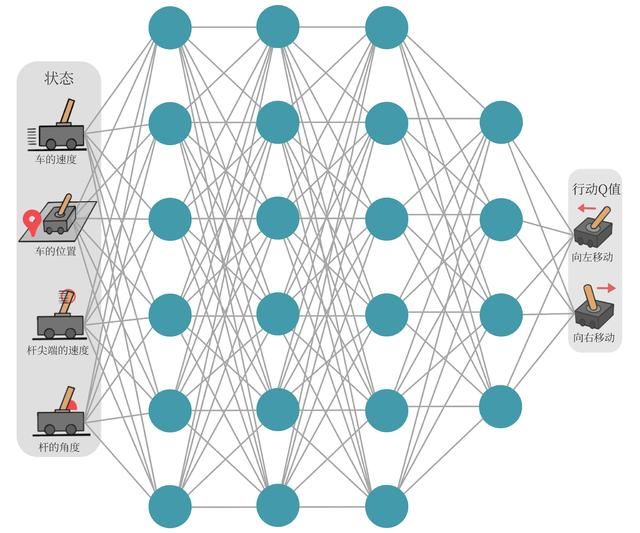
\includegraphics{images/image-0013.jpeg}
\caption{DQN 用神经网络拟合状态到各动作 Q 值的映射}
\end{figure}

\hypertarget{ux4e8cdqnux7684ux635fux5931ux51fdux6570}{%
\subsection{二、DQN的损失函数}\label{ux4e8cdqnux7684ux635fux5931ux51fdux6570}}

在传统的 Q-Learning 中，我们维护一张 \(Q\) 表。对于状态 \(s\) 和动作 \(a\)，更新规则如下：

\[
Q(s,a)\leftarrow Q(s,a)+\alpha\cdot\left[\left(r+\gamma\max_{a'}Q(s',a')\right)-Q(s,a)\right]
\]

\begin{itemize}
\tightlist
\item
  \(r+\gamma\max_{a'}Q(s',a')\) 是 TD Target（目标值），即我们认为 \(Q(s,a)\) 应该接近的值。
\item
  \(Q(s,a)\) 是 Current Estimate（当前估计值）。
\item
  物理意义：将当前的 \(Q(s,a)\) 向目标值拉近一点（步长为 \(\alpha\)）。
\end{itemize}

在 DQN 中，我们用神经网络 \(Q(s,a;\theta)\) 来拟合 \(Q\) 值。我们需要定义一个损失函数 \(L(\theta)\) 来训练网络。DQN 采用的是均方误差（MSE），目标是让网络的输出 \(Q(s,a;\theta)\) 尽可能接近 TD Target。

\[
L(\theta)=\mathbb{E}\left[\left(r+\gamma\max_{a'}Q(s',a';\theta^-)-Q(s,a;\theta)\right)^2\right]
\]

其中 \(y=r+\gamma\max_{a'}Q(s',a';\theta^-)\) 是目标值，在计算梯度时被视为常数；\(\theta^-\) 是目标网络的参数。

\hypertarget{ux4e09dqnux7684ux68afux5ea6ux66f4ux65b0}{%
\subsection{三、DQN的梯度更新}\label{ux4e09dqnux7684ux68afux5ea6ux66f4ux65b0}}

将目标值记为 \(y=r+\gamma\max_{a'}Q(s',a';\theta^-)\)，则 DQN 损失函数的梯度为：

\[
\begin{aligned}
\nabla_\theta L(\theta)
&=\nabla_\theta\left(y-Q(s,a;\theta)\right)^2\\
&=2\cdot\left(y-Q(s,a;\theta)\right)\cdot\nabla_\theta\left(-Q(s,a;\theta)\right)\\
&=-2\cdot\left[\left(r+\gamma\max_{a'}Q(s',a';\theta^-)\right)-Q(s,a;\theta)\right]\cdot\nabla_\theta Q(s,a;\theta)
\end{aligned}
\]

其中括号中的差值就是 TD Error \(\delta\)。参数更新规则（梯度下降）为：

\[
\theta\leftarrow\theta-\eta\cdot\nabla_\theta L(\theta)
\]

代入梯度后得到：

\[
\theta\leftarrow\theta+\eta\cdot2\cdot\delta\cdot\nabla_\theta Q(s,a;\theta)
\]

对比来看，Q-Learning 直接修改 \(Q(s,a)\) 的值，增加量正比于 TD Error；DQN 修改的是参数 \(\theta\)，使 \(Q(s,a;\theta)\) 的输出值沿梯度方向变化，变化幅度同样正比于 TD Error。
\#\#\# 四、经验回放

\begin{enumerate}
\def\labelenumi{\arabic{enumi}.}
\tightlist
\item
  概念
\end{enumerate}

监督学习中，我们往往假设训练数据是独立同分布的，在训练时每个batch也是随机采样的，保证了每个batch的梯度方向是对整个数据集梯度方向的一个无偏估计。但在马尔可夫决策过程（MDP）中，智能体产生的数据是一个时间序列轨迹：s\_0, a\_0, r\_0, s\_1, a\_1, r\_1,\ldots，状态s\_\{t+1\}直接依赖于s\_t和a\_t。这意味着数据高度相关，如果机器人在走迷宫，前一秒它在左下角，下一秒它大概率还在左下角附近。如果直接拿这些数据训练，神经网络会连续看到很多``左下角''的数据。数据是一个非平稳分布：随着策略pi的更新，智能体访问的状态分布也会发生变化，导致训练数据的分布本身就在变。当它极力优化当前连续片段的数据时，它会修改共享的权重，导致它``忘记''了之前在其他状态下学到的知识（和大模型推理过程中的``灾难性遗忘''亦是如此）。

因而我们引入经验回放：智能体与环境交互，每一步生成一个四元组e\_t = (s\_t, a\_t, r\_t, s\_t+1)，将这个e\_t存入固定容量的缓冲区中。在训练时刻t，我们每和环境交互一次，就从缓冲区中均匀若干次随机采样小批次的数据来进行梯度下降。

\begin{enumerate}
\def\labelenumi{\arabic{enumi}.}
\setcounter{enumi}{1}
\tightlist
\item
  优点
\end{enumerate}

打破相关性：通过随机采样，一个 batch 内的数据可能包含3天前的数据、5分钟前的数据、刚刚的数据，使得这个batch的数据分布接近于智能体的全局历史分布，而不是当前局部的一段轨迹，近似满足了独立同分布假设。

提高数据利用率：在原始Q-learning中，数据用完即弃。训练DQN网络时，每次获取新数据后，让Loss下降到接近0往往需要多次梯度下降拟合中，一个样本存入缓冲区后，可能会被多次采样用于梯度更新。这极大地提高了样本利用率（因为获取环境数据的代价通常很高）。

\begin{enumerate}
\def\labelenumi{\arabic{enumi}.}
\setcounter{enumi}{2}
\tightlist
\item
  与Dyna-Q中引入的``环境模型''的区别
\end{enumerate}

DQN不试图理解环境的运作机制，只是维护一个巨大的经验池，里面存储的是真实的元组(s\_t, a\_t, r\_t, s\_t+1)构成。每次更新参数时，从经验池中随机抽取一批曾经真实发生的数据，直接利用这些历史事实来计算损失函数并更新神经网络。

``环境模型''则维护一个函数，输入s\_t和a\_t，该函数会输出r\_t和s\_t+1。在更复杂的情境下，这个模型通常是一个神经网络。我们更新参数时，随机选择一个过去走过的(s\_t,a\_t)，但并不用过去在某一次真实发生的(r\_t,s\_t+1)，而是运用这个网络的输出值。这个函数（神经网络）具有泛化性，在高级版本中我们还可以让环境模型选择没有走过的(s\_t,a\_t)，模型可以根据学会的物理规律给出一个预测（这是经验回放做不到的，因为经验回放池里没有这一条数据），运用网络的输出值，让Q网络学习泛化性能。

\hypertarget{ux4e94ux76eeux6807ux7f51ux7edc}{%
\subsection{五、目标网络}\label{ux4e94ux76eeux6807ux7f51ux7edc}}

DQN 算法最终更新的目标是让Q(s,a)逼近r+gamma*maxQ(s',a')，由于TD误差目标本身就包含神经网络的输出，因此在更新网络参数的同时目标也在不断地改变，这非常容易造成神经网络训练的不稳定性。为了解决这一问题，DQN便使用了目标网络的思想：既然训练过程中Q网络的不断更新会导致目标不断发生改变，不如暂时先将TD目标中的Q网络固定住。为了实现这一思想，我们需要利用两套Q网络。对于损失函数：

\[
\frac{1}{2}\left[Q_w(s,a)-\left(r+\gamma\max_{a'}Q_{w^-}(s',a')\right)\right]^2
\]

原来的训练网络（主Q网络）Q\_w用于计算损失函数中的第一项，并且使用正常梯度下降方法来进行更新。目标网络Q\_w-用于计算损失函数中的第二项，其中w-表示目标网络中的参数。如果两套网络的参数随时保持一致，则仍为原先不够稳定的算法。为了让更新目标更稳定，目标网络并不会每一步都更新。具体而言，目标网络使用训练网络的一套较旧的参数，训练网络在训练中的每一步都会更新，而目标网络的参数每隔C步才会与训练网络同步一次，即。这样做使得目标网络相对于训练网络更加稳定。

当然，目标网络也不一定直接同步训练网络的值。也可以采取``软更新''：它不会大幅改动目标网络的参数，而是缓慢地将其向主Q网络的方向调整，每隔C步，计算w-\_new=τ\emph{w+(1−τ)}w-\_new。这确保了目标Q值相对稳定，为主Q网络提供了一个可靠的学习目标。

\hypertarget{ux53c2ux8003ux6587ux732e-48}{%
\subsection{参考文献}\label{ux53c2ux8003ux6587ux732e-48}}

\begin{itemize}
\tightlist
\item
  \href{https://hrl.boyuai.com/}{《动手学强化学习》}.
\item
  Mnih, V., Kavukcuoglu, K., Silver, D., et al.~(2015). \href{https://www.nature.com/articles/nature14236}{Human-level control through deep reinforcement learning}. Nature.
\end{itemize}

\clearpage

\hypertarget{double-dqn}{%
\section{Double DQN}\label{double-dqn}}

\hypertarget{ux4e00dqnux5bf9qux503cux7684ux8fc7ux9ad8ux4f30ux8ba1}{%
\subsection{一、DQN对Q值的过高估计}\label{ux4e00dqnux5bf9qux503cux7684ux8fc7ux9ad8ux4f30ux8ba1}}

DQN普遍存在过高估计Q值的问题。这是因为其更新目标为：

\[
y=r+\gamma\max_{a'}Q(s',a';w^{-})
\]

神经网络的输出Q(s',a')总是包含噪声（估计误差）。由于取max，往往最后留下的是被高估的结果，这种高估会随着贝尔曼方程的迭代不断向回传播，导致整个系统的Q值普遍虚高。假设误差epsilon服从均匀分布，我们可以推导出估计值的最大值与真实值最大值之间的期望偏差：

为了让数学推导可行，文中做了一些简化的假设，但这些假设不影响结论的普适性：

\begin{itemize}
\tightlist
\item
  \textbf{真实价值相等}：假设在状态 \(s\) 下，所有动作 \(a\) 的真实期望回报 \(Q^{*}(s,a)\) 都一样，记为 \(V^{*}(s)\)。
\item
  \textbf{为什么要这样假设}：如果真实价值本身有高有低，那么 \(\max\) 操作选到最大值是理所应当的。这里要证明的是：即使所有动作真实价值都一样，仅仅因为有噪声，\(\max\) 操作也会导致评估结果偏高。
\item
  \textbf{噪声分布}：神经网络的估算误差 \(\epsilon_a=Q_{w^{-}}(s,a)-V^{*}(s)\) 服从区间 \([-1,1]\) 上的均匀分布，且 \(\mathbb{E}[\epsilon_a]=0\)。
\item
  \textbf{独立性}：不同动作的估算误差相互独立。
\item
  \textbf{动作数量}：动作空间大小为 \(m\)。
\end{itemize}

我们的目标是计算：在这种情况下，神经网络估算出的最大值 \(\max_a Q_{w^{-}}(s,a)\) 比真实值 \(V^{*}(s)\) 高出多少，即计算期望 \(\mathbb{E}[\max_a\epsilon_a]\)。

因为 \(\epsilon_a\) 服从 \([-1,1]\) 上的均匀分布，其分布函数为：

\[
P(\epsilon_a\le x)=
\begin{cases}
0, & x\le -1\\
\frac{1+x}{2}, & x\in(-1,1)\\
1, & x\ge 1
\end{cases}
\]

现在需要求 \(m\) 个误差中的最大值 \(\max_a\epsilon_a\) 的分布。如果 \(m\) 个数的最大值都小于等于 \(x\)，那么这 \(m\) 个数每一个都必须小于等于 \(x\)。由于它们相互独立，联合概率等于各自概率的乘积：

\[
P(\max_a\epsilon_a\le x)
=\prod_{a=1}^{m}P(\epsilon_a\le x)
=(\frac{1+x}{2})^{m}
\]

最后一步是求这个``最大误差''的数学期望。期望定义为 \(\mathbb{E}[X]=\int x\cdot p(x)dx\)，其中 \(p(x)\) 是概率密度函数，也就是分布函数的导数。文中给出的积分公式为：

\[
\mathbb{E}[\max_a\epsilon_a]
=\int_{-1}^{1}x\cdot\frac{d}{dx}P(\max_a\epsilon_a\le x)dx
\]

积分结果为：

\[
=[(\frac{x+1}{2})^{m}\frac{mx-1}{m+1}]_{-1}^{1}
\]

最终得到：

\[
\mathbb{E}[\max_a Q_{w^{-}}(s,a)-\max_{a'}Q^{*}(s,a')]=\frac{m-1}{m+1}
\]

如果只有一个动作可以选择，没有max操作，那么随着每一次采样：

假设只有一个动作 \(a_1\)：

\begin{itemize}
\tightlist
\item
  \textbf{真实情况}：它的价值是 \(0\)。
\item
  \textbf{噪声}：服从 \([-1,1]\) 的均匀分布。这意味着有时会估成 \(0.8\)（高估），有时会估成 \(-0.9\)（低估）。
\end{itemize}

虽然单次看有误差，但如果尝试很多次并求平均：

\[
\mathcjk{平均误差}=\frac{(+0.8)+(-0.9)+(+0.1)+(-0.5)+\cdots}{N}\approx 0
\]

结论是：因为噪声是对称的，正向误差和负向误差会相互抵消，所以平均来看既没有过高估计，也没有过低估计，这称为无偏估计。

如果有两个动作 \(a_1\) 和 \(a_2\)，两者真实价值都是 \(0\)。Q-Learning 的 \(\max\) 操作会强迫系统挑选估值最高的那个动作。例如：

\begin{itemize}
\tightlist
\item
  第 1 次尝试：\(a_1\) 的噪声为 \(-0.5\)，\(a_2\) 的噪声为 \(+0.8\)，\(\max\) 操作选中 \(+0.8\)，结果是过高估计 \(+0.8\)。
\item
  第 2 次尝试：\(a_1\) 的噪声为 \(+0.3\)，\(a_2\) 的噪声为 \(-0.9\)，\(\max\) 操作选中 \(+0.3\)，结果是过高估计 \(+0.3\)。
\end{itemize}

动作越多，过高估计的偏差就越接近噪声的上界（这里是1）。因为动作越多，越容易每次都``运气好''碰上一个正向误差特别大的噪声，而max操作一定会选中它。

\hypertarget{ux4e8cdouble-dqn}{%
\subsection{二、Double DQN}\label{ux4e8cdouble-dqn}}

前面我们提过DQN高估Q值的问题。归根到底，这种误差来源于我们在计算目标值时，使用同一个网络（目标网络）来做两件事：选择哪个动作是最好的；评估这个动作的价值是多少。这样，每次动作都会选择高估的样本（因为高估所以选择），而每一次更新都直接运用对选择动作的价值估计（因为选择所以用于更新），导致每一次更新都写入了被高估的值。

Double DQN打破了这个链条：使用训练网络w来决定哪个动作最好，因为训练网络更新最及时，能反映最新的策略；使用目标网络w-来计算选定动作的Q值。Double DQN的更新目标变为：

\[
y_{DDQN}=r+\gamma Q(s',\arg\max_{a'}Q(s',a';w);w^{-})
\]

其中 \(\arg\max_{a'}Q(s',a';w)\) 表示由训练网络选择动作。
如果训练网络w因为噪声错误地认为某个动作最好（高估了），通过将其放入目标网络w-进行评估，由于两个网络的参数不同，w-极有可能不会同时也高估这个动作。这样就抵消了大部分的过高估计偏差。

\hypertarget{ux53c2ux8003ux6587ux732e-49}{%
\subsection{参考文献}\label{ux53c2ux8003ux6587ux732e-49}}

\begin{itemize}
\tightlist
\item
  van Hasselt, H., Guez, A., \& Silver, D. (2016). \href{https://arxiv.org/abs/1509.06461}{Deep Reinforcement Learning with Double Q-learning}. AAAI 2016.
\end{itemize}

\clearpage

\hypertarget{dueling-dqn}{%
\section{Dueling DQN}\label{dueling-dqn}}

DQN中，\(Q\) 是一个同时由状态 \(s\) 和动作 \(a\) 决定的函数。但在某些状态下，智能体只需要知道``现在的环境好不好''（\(V\) 值），而不关心具体动作的差异；而在需要通过做动作来避险或得分时，才需要关心``哪个动作比平均水平好''（\(A\) 值）。如果我们将两者分开建模，\(V(s)\) 专门负责看大局，评估当前环境好不好；\(A(s,a)\) 专门负责看细节，评估在当前环境下，哪个动作比其他动作好，好多少。这种解耦使得 \(V(s)\) 可以在每一个样本中都被学习更新（因为无论选哪个动作，\(V(s)\) 都是基础），从而大幅提升了训练效率。

\begin{figure}[htbp]
\centering
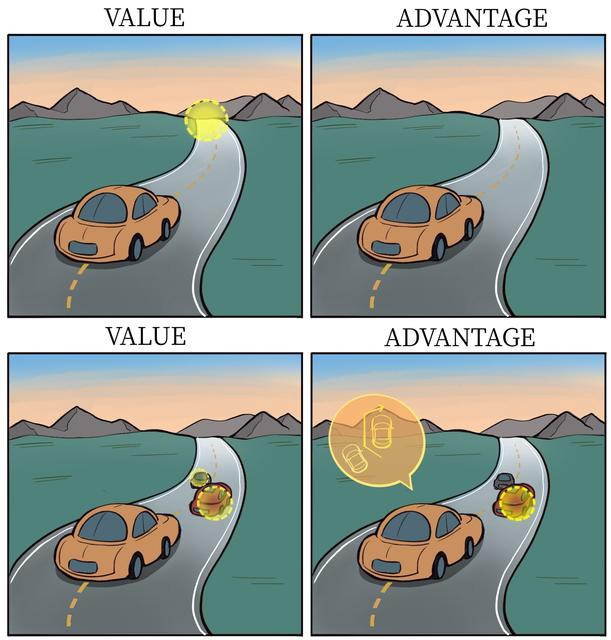
\includegraphics{images/image-0014.jpeg}
\caption{Dueling DQN 中状态价值和动作优势的直观区别}
\end{figure}

场景 A（大直道，前方无车）：此时通过屏幕（状态 \(s\)），可以判断当前局势较稳，在这个状态下大概率能得高分。此时，无论稍微向左打方向盘，还是向右打方向盘（动作 \(a\)），对最终得分的影响都较小。

\begin{itemize}
\tightlist
\item
  结论：此时 \(V(s)\)（状态价值）很高，而 \(A(s,a)\)（动作优势）的差异很小。神经网络不必费力学习每个动作的具体数值，只需要知道``这里不错''即可。
\end{itemize}

场景 B（前方有障碍物，必须急转弯）：此时状态 \(s\) 很危险，如果不操作好就会撞车。

\begin{itemize}
\tightlist
\item
  结论：此时动作选择非常重要，向左转可能存活，向右转可能失败。这时 \(A(s,a)\)（动作优势）的差异很大。
  从而我们把Q函数拆分如下：
\end{itemize}

\[
Q(s,a;\theta,\alpha,\beta)=V(s;\theta,\beta)+A(s,a;\theta,\alpha)
\]

\begin{itemize}
\tightlist
\item
  \(\theta\)：共享参数（卷积层），负责从图像中提取边缘、形状、物体位置等通用特征。这些特征既对判断局势有用，也对选择动作有用。
\item
  \(\beta\)：价值流参数（全连接层），将特征映射为一个标量 \(V\)。
\item
  \(\alpha\)：优势流参数（全连接层），将特征映射为一个向量 \(A\)，维度为动作数。
  但问题在于，我们计算和更新的都是 \(Q\) 值，怎么从 \(Q\) 值中求出 \(V\) 和 \(A\)？
\end{itemize}

我们可以获取同一个状态 \(s\) 上的所有动作 \(a'\)（遍历），各个动作 \(Q\) 值的相对大小关系也就是它们的 \(A\) 值相对大小。一个方案是对于给定 \(s\)，取让 \(Q(s,a')\) 最大的动作 \(a^*\)，设 \(A(s,a^*)=0\)（最大动作优势值），\(V(s)=Q(s,a^*)\)，则：

方案 A：Max 约束（理论最优）

\[
Q(s,a)=V(s)+(A(s,a)-\max_{a'}A(s,a'))
\]

\begin{itemize}
\tightlist
\item
  数学含义：强制让最大的优势值为 \(0\)。
  另一方案是取所有动作优势值的平均值为0：
\end{itemize}

方案 B：Mean 约束（工程最优）

\[
Q(s,a)=V(s)+(A(s,a)-\frac{1}{|\mathcal{A}|}\sum_{a'}A(s,a'))
\]

\begin{itemize}
\item
  数学含义：强制让所有动作的优势值之和为 \(0\)，也就是平均值为 \(0\)。
\item
  为什么更好：\(\max\) 操作是非线性操作，梯度只在最大值处传递，其他位置梯度为 \(0\)；而 mean 操作涉及所有动作的求和，梯度可以平滑地回传给每一个动作优势输出节点。
\item
  抗噪性：均值对异常值不那么敏感，能让网络训练更平稳。
  这样虽然不严格满足贝尔曼最优方程，但在工程实现上更优。原因如下：
\item
  数学含义：强制让所有动作的优势值之和为 \(0\)（即平均值为 \(0\)）。
\item
  为什么更好：

  \begin{itemize}
  \tightlist
  \item
    梯度稳定性：\(\max\) 操作是一个非线性操作，梯度只在最大值处传递，其他位置梯度为 \(0\)。而 mean 操作涉及所有动作的求和，梯度可以平滑地回传给每一个动作的优势输出节点。
  \item
    抗噪性：均值对异常值不那么敏感，能让网络训练更平稳。
  \end{itemize}
\end{itemize}

\hypertarget{ux53c2ux8003ux6587ux732e-50}{%
\subsection{参考文献}\label{ux53c2ux8003ux6587ux732e-50}}

\begin{itemize}
\tightlist
\item
  Wang, Z., Schaul, T., Hessel, M., van Hasselt, H., Lanctot, M., \& de Freitas, N. (2016). \href{https://arxiv.org/abs/1511.06581}{Dueling Network Architectures for Deep Reinforcement Learning}. ICML 2016.
\item
  \href{https://hrl.boyuai.com/}{《动手学强化学习》}.
\end{itemize}

\clearpage

\hypertarget{ux6709ux6a21ux578bux7684dqnux7b97ux6cd5}{%
\section{有模型的DQN算法}\label{ux6709ux6a21ux578bux7684dqnux7b97ux6cd5}}

\hypertarget{ux4e00ux7ecfux9a8cux56deux653eux65e0ux6cd5ux89e3ux51b3ux68afux5ea6ux4f20ux64adux7f13ux6162ux7684ux95eeux9898}{%
\subsection{一、经验回放无法解决梯度传播缓慢的问题}\label{ux4e00ux7ecfux9a8cux56deux653eux65e0ux6cd5ux89e3ux51b3ux68afux5ea6ux4f20ux64adux7f13ux6162ux7684ux95eeux9898}}

在标准的 Q-Learning 和 DQN 中，更新目标是：

\[
y=r+\gamma \max_{a'}Q(s',a')
\]

\begin{itemize}
\tightlist
\item
  这被称为 TD(0)。
\item
  在这个公式里，\(Q(s,a)\) 的价值更新只利用了一步之后的真实奖励 \(r\) 和下一时刻的估计 \(Q(s',a')\)。
\item
  后果：假设你在走迷宫，只有到达终点才有奖励。

  \begin{itemize}
  \tightlist
  \item
    第 1 次成功：只有终点前的最后一步状态更新了 Q 值。
  \item
    第 2 次成功：倒数第二步的状态通过倒数第一步的 Q 值更新了。
  \item
    \ldots{}
  \end{itemize}
\end{itemize}

比如说，如果我们只获得了最后一步的环境数据，没有倒数第二步的奖励值，那么在经验回放里也不会出现倒数第二步，进而梯度仍然无法通过该路径传播到前面的步骤。

经验回放（Experience Replay）相当于``翻看日记''：

\begin{itemize}
\tightlist
\item
  本质：它存储的是真实发生过的数据。
\item
  机制：你有一个数据库（Buffer），里面原封不动地记录了你在过去某个时刻做了什么、环境反馈了什么。
\item
  数据来源：真实的物理世界。
\item
  可靠性：绝对真实（Ground Truth）。只要环境本身没有发生物理规则的改变（比如摩擦力突然变了），缓冲区里的 \((s,a,r,s')\) 永远是符合物理规律的。
\item
  局限性：只能回放已经见过的场景。你无法通过回放去探索那些你从未去过的地方。
\end{itemize}

Dyna-Q 的环境模型（Environment Model）相当于``脑补模拟''：

\begin{itemize}
\tightlist
\item
  本质：它是一个被学习出来的函数（或者神经网络）。
\item
  机制：你通过观察真实数据，训练了一个模型 \(M(s,a)\to(r,s')\)。训练好后，你给它一个 \((s,a)\)，它通过计算预测出一个 \((r,s')\)。
\item
  数据来源：模型的预测（Hallucination/Prediction）。
\item
  可靠性：存在偏差（Model Bias）。如果模型没学好，它预测的结果可能是错的。例如，模型可能错误地认为``撞墙不会扣分''，基于这个错误模型的训练会导致错误的策略。
\item
  优势：泛化能力。如果使用神经网络作为模型，理论上它可以预测那些你未曾精确到达但与已知状态相似的状态的结果。
\end{itemize}

为什么说经验回放是``非参数化模型''？

在统计学中，非参数方法是指不假设数据服从某种特定分布，而是直接利用数据本身。

\begin{itemize}
\tightlist
\item
  Dyna-Q 试图学习 \(P(s'|s,a)\) 的参数（参数化）。
\item
  经验回放不学参数，直接拿样本代表分布（非参数化）。从这个角度看，经验回放就是一个不需要训练、不会产生预测偏差、但体积巨大的环境模型。
\end{itemize}

\hypertarget{ux4e8cn-step-td-learningux52a0ux901fux5df2ux83b7ux5f97ux7684ux68afux5ea6ux6570ux636eux7684ux4f20ux64ad}{%
\subsection{二、N-step TD Learning：加速已获得的梯度数据的传播}\label{ux4e8cn-step-td-learningux52a0ux901fux5df2ux83b7ux5f97ux7684ux68afux5ea6ux6570ux636eux7684ux4f20ux64ad}}

不使用环境模型，但改变目标函数的视野。DQN 可以很容易地扩展为 N-step DQN。我们不再只看一步，而是看 \(n\) 步：

\[
y=r_t+\gamma r_{t+1}+\cdots+\gamma^{n}\max_{a'}Q(s_{t+n},a')
\]

\begin{itemize}
\tightlist
\item
  作用：一次更新，奖励信号直接回传 \(n\) 步。
\item
  优缺点：比单步快，但如果 \(n\) 太大，方差（Variance）会变大。
\end{itemize}

\hypertarget{ux4e09model-based-deep-rldyna-qux7684ux771fux6b63ux7ee7ux627fux8005}{%
\subsection{三、Model-Based Deep RL：Dyna-Q的真正继承者}\label{ux4e09model-based-deep-rldyna-qux7684ux771fux6b63ux7ee7ux627fux8005}}

这才是真正对应你提到的 Dyna-Q 思想的方法。这类算法会训练一个世界模型（World Model），通常包含：

\begin{itemize}
\tightlist
\item
  动力学模型：预测 \(s_{t+1}=f(s_t,a_t)\)。
\item
  奖励模型：预测 \(r_t=R(s_t,a_t)\)。
\end{itemize}

DQN 采用经验回放，是因为在处理高维输入（如图像）时，``记住过去''比``预测未来''容易得多，也准确得多。训练一个能生成逼真游戏画面的视频生成模型（基于世界模型）比单纯训练一个玩游戏的Q网络要难得多，因此只有低维或简单环境下才会用model-based方法（如Dyna-Q）。然而，学习环境规律带来的泛化优势无可比拟，随着算力的提升和生成式AI的发展，现在的 AI 已经开始能够比较准确地``想象''未来了。因此，基于世界模型的Model-Based RL（如Dreamer算法）正在重新回归主流，试图取代或增强仅靠``回忆''（经验回放）的算法。

Dyna-Style Deep RL（如 MBPO - Model-Based Policy Optimization）：

\begin{itemize}
\tightlist
\item
  训练一个神经网络来模拟环境动力学。
\item
  在训练 Q 网络（或策略网络）时，不仅使用真实环境采样的数据（Experience Replay），还使用从模型中生成的虚拟数据。
\item
  效果：这完全复刻了 Dyna-Q 的逻辑，极大地提高了样本效率。在 MuJoCo 等控制任务上，MBPO 只需极少的真实交互就能达到很好的效果。
\end{itemize}

Latent Dynamics Models（如 Dreamer、MuZero）：

\begin{itemize}
\tightlist
\item
  Dreamer：在图像输入的任务中，先将图像编码为隐空间（Latent Space）的状态，在隐空间中学习世界模型。然后在``梦境''（隐空间的模拟序列）中训练 Actor-Critic。
\item
  MuZero：DeepMind 的算法，它不需要重构像素，而是直接在隐空间进行规划（Planning），结合了蒙特卡洛树搜索（MCTS）和模型学习。
\end{itemize}

\hypertarget{ux53c2ux8003ux6587ux732e-51}{%
\subsection{参考文献}\label{ux53c2ux8003ux6587ux732e-51}}

\begin{itemize}
\tightlist
\item
  Mnih, V., Kavukcuoglu, K., Silver, D., et al.~(2015). \href{https://doi.org/10.1038/nature14236}{Human-level control through deep reinforcement learning}. Nature.
\item
  Sutton, R. S. (1990). \href{https://doi.org/10.1016/B978-1-55860-141-3.50030-4}{Integrated Architectures for Learning, Planning, and Reacting Based on Approximating Dynamic Programming}. ICML 1990.
\item
  Janner, M., Fu, J., Zhang, M., \& Levine, S. (2019). \href{https://arxiv.org/abs/1906.08253}{When to Trust Your Model: Model-Based Policy Optimization}. NeurIPS 2019.
\item
  Hafner, D., Lillicrap, T., Ba, J., \& Norouzi, M. (2020). \href{https://openreview.net/forum?id=S1lOTC4tDS}{Dream to Control: Learning Behaviors by Latent Imagination}. ICLR 2020.
\item
  Schrittwieser, J., Antonoglou, I., Hubert, T., et al.~(2020). \href{https://doi.org/10.1038/s41586-020-03051-4}{Mastering Atari, Go, chess and shogi by planning with a learned model}. Nature.
\end{itemize}

\clearpage
